%!TEX root=../main.tex


\section*{Аннотация}

DSLab - программный фреймворк для имитационного моделирования и тестирования распределенных систем.

В проекте используется дискретно-событийный подход описания моделей и приложений, где события обрабатываются в пользовательских функциях (callback-ах). В рамках проекта предстоит добавить возможность управлять событиями асинхронно.


\section{Описание проекта и постановка задачи}

\subsection{Устройство DSLab}

В силу широты охвата областей применения фреймворка он организован в виде набора слабо связанных программных модулей, использование которых будет осуществляться через их API. Это даст возможность пользователям фреймворка (исследователям, разработчикам, преподавателям) гибким образом собирать из модулей решения под свои цели, например симуляторы для конкретных типов систем или постановок задач.

Входящие в состав фреймворка модули можно условно разделить на три типа:
\begin{enumerate}
    \item 
    Базовые, функциональность которых используется остальными модулями (например, реализация дискретно-событийного моделирования)
    \item
    Универсальные, функциональность которых может быть использована в различных предметных областях (например, модели сети);
    \item
    Специализированные, которые заточены под определенную предметную область (например, библиотеки для моделирования облачных инфраструктур, исследования алгоритмов планирования заданий на кластерах или тестирования решений учебных заданий).
\end{enumerate}

Архитектуру DSLab можно схематично представить в виде трех слоев (Рис. \ref{dslab_arc}), включающих модули соответствующего типа. На рисунке также указаны текущие модули и зависимости между ними. Зависимости от dslab-core (от него зависят все имеющиеся универсальные и специализированные модули) не указаны, чтобы не загромождать рисунок. Таким образом, модули могут зависеть от модулей с нижних слоев, но не наоборот.

\begin{figure}[H]
    \centering
    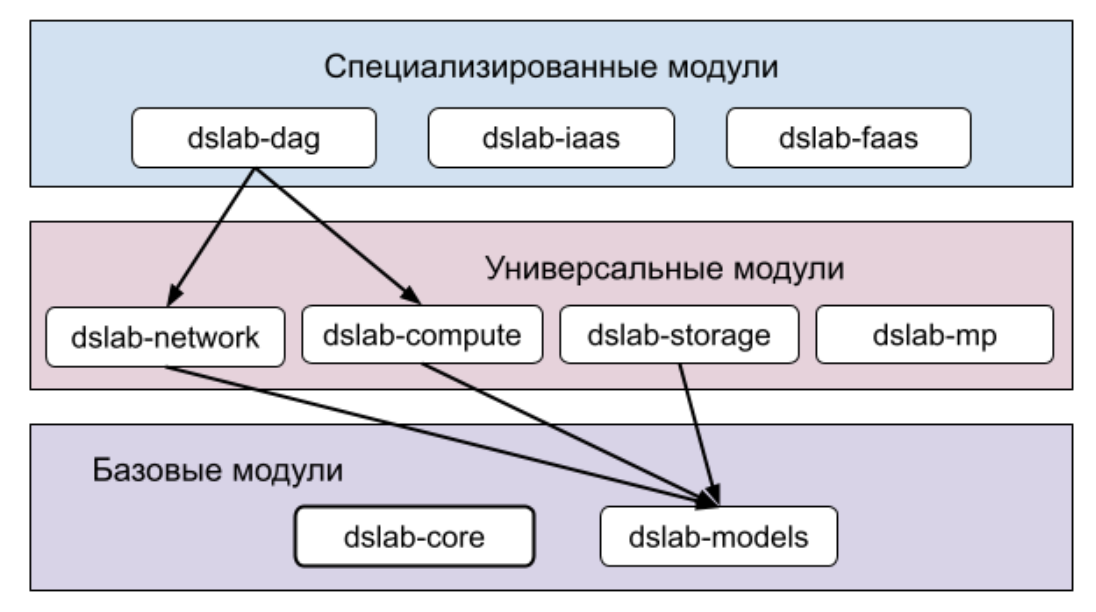
\includegraphics[width=0.7\linewidth]{images/dslab_arc.png}
    \caption{Архитектура DSLab}
    \label{dslab_arc}
\end{figure}


% TODO \cite{dslab-docs}

Таким образом пользователь при разработке собственной симмуляции может либо использовать уже готовые разработанные компоненты, либо реализовывать свои и произвольно их свзяывать. 

Основным процессом создания симуляции является создание событий и написание процессов реагирования на них. Каждое событие представляет из себя следующую структуру: 
\begin{enumerate}
    \item идентификатор события 
    \item идентификатор компонента, создавшего событие 
    \item идентификатор компонента, которому это событие предназначено доставить 
    \item внутреннее время, когда событие должно наступить
    \item прозвольные данные события (<<полезная нагрузка>>)
\end{enumerate}

Таким образом в процессе симуляции разные компоненты генерируют события друг для друга и с помощью самого базового модуля dslab-core обмениваются ими.

В текущей реализации проект поддерживает одну общую схему реагирования на события -- через написание хэндлеров. 

\subsection{Цель}

Добавить возможность использовать асинхронность как альтернативу текущей модели программирования с событиями и callback-ами.

\section{Актуальность и значимость}

\section{Существующие работы и решения}

\section{Предлагаемые подходы и методы} 

\section{Ожидаемые результаты}

Поддержана возможность реализовывать алгоритмы в DSLab используя асинхронность. 

В проект добавлены примеры кода, документация по использованию реализованных методов.

\section{План работ}